\section{Implementación}\label{implementacion}

Un sistema de captura de movimiento con las características necesarias para cumplir el objetivo de este proyecto debe estar formado por cuatro bloques generales: \emph{calibración}, \emph{detección de marcadores}, \emph{reconstrucción} y \emph{seguimiento}. En la Figura \ref{bloquesSist} se muestra un esquema del sistema a implementar.

\begin{figure}[ht!]
\centering
\hspace{-0.5cm}
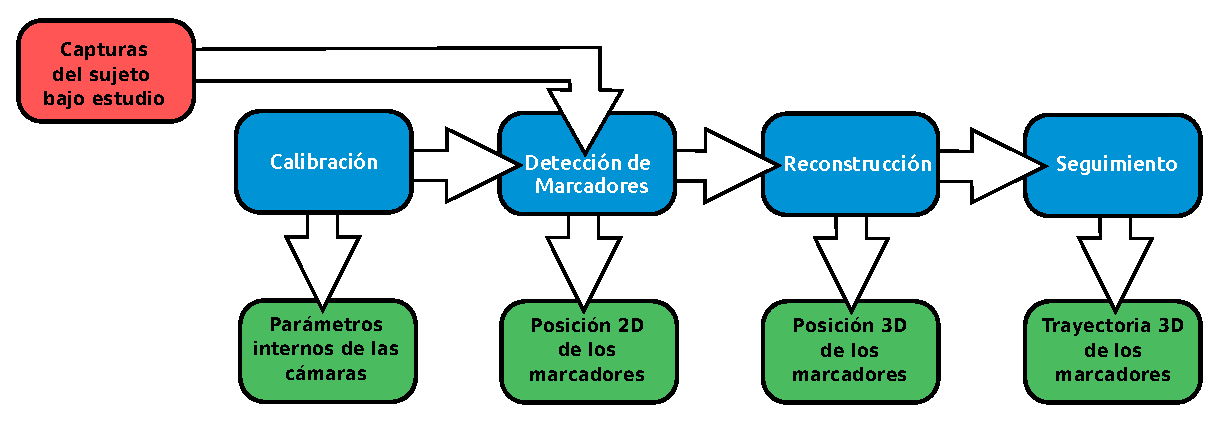
\includegraphics[scale=0.5]{imagenes/Sistema_completo/Diagrama_de_bloques.eps}
\caption{Diagrama de bloques del sistema completo.}
\label{bloquesSist}
\end{figure}

Es importante destacar el hecho de poder separar el sistema en bloques independientes,
%. Esto asegura que el funcionamiento de uno de ellos no dependa del funcionamiento de otro. Por otro lado, da la posibilidad que en etapas futuras se pueda realizar el estudio de uno de los bloques de la Figura \ref{bloquesSist} individualmente y así poder modificarlo u optimizarlo sin afectar al resto.
esto permite en etapas futuras modificar u optimizar cada bloque individualmente sin afectar al resto.

En los capítulos que siguen, se explicará el funcionamiento de cada bloque de forma detallada, así como su implementación y el análisis de resultados de cada uno de ellos.